\documentclass[10pt]{standalone}
\usepackage{mathptmx}
\usepackage{times}
\usepackage{amsmath}
\usepackage{graphicx}
\usepackage{tikz}
\usetikzlibrary{positioning,arrows.meta,fit,calc}
\begin{document}
\resizebox{16.51cm}{!}{% Figure 4.3, reference-matched style: grey material, black contours, discrete
% particles, blue offsets and a restrained blue gradient-return path.
% Regular stage titles above long, thin arrows follow the user's second reference.
% Schematic geometry only; the dashed curve is the 3D placement target.
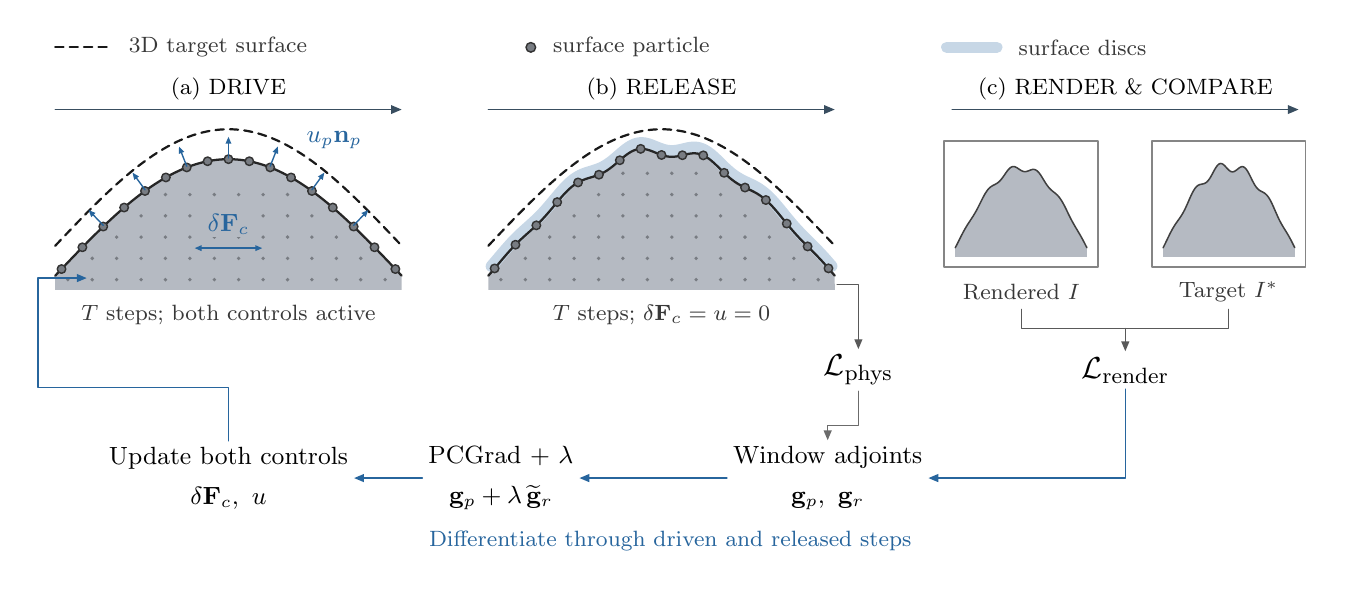
\begin{tikzpicture}[
  font=\fontsize{8.7}{10.5}\selectfont,
  line cap=round,line join=round,
  declare function={
    shape(\x)=0.18+1.48*sin(180*\x/4.4);
    slope(\x)=1.057*cos(180*\x/4.4);
    settled(\x)=shape(\x)+0.10*sin(180*\x/4.4)+0.065*sin(430*\x)*sin(180*\x/4.4);
    targetshape(\x)=shape(\x)+0.38;
  },
  stage/.style={draw=gparrow,line width=0.45pt,-{Triangle[length=1.35mm,width=1.1mm]}},
  state/.style={draw=black!65,line width=0.5pt,-{Triangle[length=1.25mm,width=1.0mm]}},
  gradient/.style={draw=gpblue,line width=0.5pt,-{Triangle[length=1.25mm,width=1.0mm]}},
  physicsgrad/.style={draw=black!58,line width=0.5pt,-{Triangle[length=1.25mm,width=1.0mm]}},
  offset/.style={draw=gpblue,line width=0.5pt,-{Triangle[length=0.88mm,width=0.70mm]}},
  target/.style={draw=black!90,line width=0.8pt,dash pattern=on 3pt off 2.2pt},
  boundary/.style={draw=black!85,line width=0.82pt},
  surfaceparticle/.style={fill=gpdot,draw=black!80,line width=0.52pt},
  heading/.style={font=\fontsize{8.2}{10.0}\selectfont,align=center},
  note/.style={font=\fontsize{8.0}{9.5}\selectfont,align=center,text=black!78},
  operation/.style={align=center,font=\fontsize{8.8}{10.5}\selectfont,inner sep=2pt},
]
\definecolor{gpbody}{RGB}{181,186,194}
\definecolor{gpdot}{RGB}{120,124,130}
\definecolor{gpblue}{RGB}{39,101,157}
\definecolor{gparrow}{RGB}{57,78,96}
\path[use as bounding box] (0,0.15) rectangle (16.55,7.00);

% Legend follows the user's reference; no coloured header bars or UI cards.
\draw[target] (0.35,6.75) -- (1.03,6.75);
\node[note,anchor=west] at (1.16,6.75) {3D target surface};
\filldraw[surfaceparticle] (6.39,6.75) circle (0.061);
\node[note,anchor=west] at (6.55,6.75) {surface particle};
\draw[gpblue!26,line width=4pt] (11.67,6.75) -- (12.31,6.75);
\node[note,anchor=west] at (12.46,6.75) {surface discs};

\node[heading] at (2.55,6.22) {(a) DRIVE};
\node[heading] at (8.05,6.22) {(b) RELEASE};
\node[heading] at (13.94,6.22) {(c) RENDER \& COMPARE};
\draw[stage] (0.35,5.96) -- (4.75,5.96);
\draw[stage] (5.85,5.96) -- (10.25,5.96);
\draw[stage] (11.74,5.96) -- (16.14,5.96);

% Large material cross-section: both controls act on this same particle body.
\begin{scope}[shift={(0.35,3.67)}]
  \fill[gpbody] (0,0) -- plot[domain=0:4.4,samples=100] (\x,{shape(\x)}) -- (4.4,0) -- cycle;
  \foreach \i in {0,...,13} {
    \foreach \j in {0,...,5} {
      \pgfmathsetmacro\px{0.16+0.31*\i}
      \pgfmathsetmacro\py{0.13+0.27*\j}
      \pgfmathsetmacro\limit{shape(\px)-0.18}
      \ifdim\py pt<\limit pt
        \fill[gpdot] (\px,\py) circle (0.024);
      \fi
    }
  }
  \draw[boundary] plot[domain=0:4.4,samples=100] (\x,{shape(\x)});
  \draw[target] plot[domain=0:4.4,samples=100] (\x,{targetshape(\x)});
  \foreach \i in {0,...,16} {
    \pgfmathsetmacro\px{0.08+0.265*\i}
    \filldraw[surfaceparticle] (\px,{shape(\px)}) circle (0.054);
  }
  % A normal offset is local and does not project the surface onto the target.
  \foreach \px in {0.61,1.14,1.67,2.20,2.73,3.26,3.79} {
    \pgfmathsetmacro\norm{sqrt(1+slope(\px)^2)}
    \draw[offset] (\px,{shape(\px)+0.015}) -- ++({-0.27*slope(\px)/\norm},{0.27/\norm});
  }
  % Balanced interior arrows indicate the stress-based bulk control.
  \draw[gpblue,line width=0.5pt,{Triangle[length=0.88mm,width=0.70mm]}-{Triangle[length=0.88mm,width=0.70mm]}]
    (1.77,0.53) -- (2.63,0.53);
  \node[fill=gpbody,inner sep=1pt,text=gpblue] at (2.20,0.83) {$\delta\mathbf{F}_c$};
  \node[text=gpblue,anchor=west,inner sep=1pt] at (3.15,1.90) {$u_p\mathbf{n}_p$};
\end{scope}
\node[note] at (2.55,3.35) {$T$ steps; both controls active};

% Release carries the same material state forward with no control actuation.
\begin{scope}[shift={(5.85,3.67)}]
  \fill[gpbody] (0,0) -- plot[domain=0:4.4,samples=150] (\x,{settled(\x)}) -- (4.4,0) -- cycle;
  \foreach \i in {0,...,13} {
    \foreach \j in {0,...,5} {
      \pgfmathsetmacro\px{0.16+0.31*\i}
      \pgfmathsetmacro\py{0.13+0.27*\j}
      \pgfmathsetmacro\limit{settled(\px)-0.18}
      \ifdim\py pt<\limit pt
        \fill[gpdot] (\px,\py) circle (0.024);
      \fi
    }
  }
  \draw[gpblue!26,line width=4.2pt] plot[domain=0.04:4.36,samples=150] (\x,{settled(\x)+0.075});
  \draw[boundary] plot[domain=0:4.4,samples=150] (\x,{settled(\x)});
  \draw[target] plot[domain=0:4.4,samples=100] (\x,{targetshape(\x)});
  \foreach \i in {0,...,16} {
    \pgfmathsetmacro\px{0.08+0.265*\i}
    \filldraw[surfaceparticle] (\px,{settled(\px)}) circle (0.054);
  }
\end{scope}
\node[note] at (8.05,3.35) {$T$ steps; $\delta\mathbf{F}_c=u=0$};

% Stylized image planes retain the geometry's visual language. Not measured images.
\draw[black!48,line width=0.55pt] (11.64,3.96) rectangle (13.59,5.56);
\draw[black!48,line width=0.55pt] (14.28,3.96) rectangle (16.23,5.56);
\begin{scope}[shift={(11.78,4.09)},xscale=0.38,yscale=0.64]
  \fill[gpbody] (0,0) -- plot[domain=0:4.4,samples=100] (\x,{settled(\x)}) -- (4.4,0) -- cycle;
  \draw[black!75,line width=0.55pt] plot[domain=0:4.4,samples=100] (\x,{settled(\x)});
\end{scope}
\begin{scope}[shift={(14.42,4.09)},xscale=0.38,yscale=0.64]
  \fill[gpbody] (0,0) -- plot[domain=0:4.4,samples=100] (\x,{shape(\x)+0.13*sin(180*\x/4.4)+0.10*sin(430*\x)*sin(180*\x/4.4)})
    -- (4.4,0) -- cycle;
  \draw[black!75,line width=0.55pt] plot[domain=0:4.4,samples=100]
    (\x,{shape(\x)+0.13*sin(180*\x/4.4)+0.10*sin(430*\x)*sin(180*\x/4.4)});
\end{scope}
\node[note] at (12.62,3.65) {Rendered $I$};
\node[note] at (15.25,3.65) {Target $I^\ast$};
\draw[black!65,line width=0.6pt] (12.62,3.42) -- (12.62,3.18) -- (15.25,3.18) -- (15.25,3.42);
\node[operation,font=\fontsize{11}{12}\selectfont] (renderloss) at (13.94,2.65) {$\mathcal{L}_{\mathrm{render}}$};
\draw[state] (13.94,3.18) -- (renderloss.north);

% A slim feedback rail. Each loss gets its own adjoint before gradient combination.
\node[operation] (update) at (2.55,1.28) {Update both controls\\[4pt]$\delta\mathbf{F}_c,\ u$};
\node[operation] (combine) at (6.01,1.28) {PCGrad + $\lambda$\\[4pt]$\mathbf{g}_p+\lambda\,\widetilde{\mathbf{g}}_r$};
\node[operation] (adjoint) at (10.16,1.28) {Window adjoints\\[4pt]$\mathbf{g}_p,\ \mathbf{g}_r$};
\draw[gradient] (renderloss.south) -- (13.94,1.28) -- (adjoint.east);
\node[operation,font=\fontsize{11}{12}\selectfont] (physloss) at (10.55,2.65) {$\mathcal{L}_{\mathrm{phys}}$};
\draw[state] (10.28,3.74) -- (10.55,3.74) -- (physloss.north);
\draw[physicsgrad] (physloss.south) -- (10.55,1.95) -- (10.16,1.95) -- (adjoint.north);
\draw[gradient] (adjoint.west) -- (combine.east);
\draw[gradient] (combine.west) -- (update.east);
\draw[gradient] (update.north) -- (2.55,2.43) -- (0.13,2.43) -- (0.13,3.82) -- (0.75,3.82);
\node[note,text=gpblue] at (8.16,0.48) {Differentiate through driven and released steps};
\end{tikzpicture}
}
\end{document}
